\documentclass[12pt,a4paper]{article}
\usepackage{amsmath,amsthm,amssymb,mathtools}
\usepackage{tikz}
\usetikzlibrary{arrows.meta,positioning,shapes.geometric,calc,fit,backgrounds}
\usepackage{graphicx}
\usepackage{booktabs,tabularx,multirow}
\usepackage[ruled,vlined,linesnumbered]{algorithm2e}
\usepackage[most]{tcolorbox}
\usepackage{hyperref}
\usepackage[capitalize,noabbrev]{cleveref}
\usepackage[margin=1in]{geometry}
\usepackage{fancyhdr}
\usepackage{enumitem}
\usepackage{xcolor}
\newtcolorbox{keyinsight}[1][]{colback=blue!5!white,colframe=blue!75!black,fonttitle=\bfseries,title=Key Insight,#1}
\newtcolorbox{example}[1][]{colback=green!5!white,colframe=green!75!black,fonttitle=\bfseries,title=Example,#1}
\newtcolorbox{warningbox}[1][]{colback=red!5!white,colframe=red!75!black,fonttitle=\bfseries,title=Warning,#1}
\newtheorem{theorem}{Theorem}[section]
\newtheorem{lemma}[theorem]{Lemma}
\newtheorem{definition}{Definition}[section]
\newtheorem{remark}{Remark}[section]

% -------------------------------------------------------
% Header / Footer
% -------------------------------------------------------
\pagestyle{fancy}
\fancyhf{}
\rhead{Deep Learning -- Session 14}
\lhead{Popular CNN Architectures}
\cfoot{\thepage}

\hypersetup{
  colorlinks=true,
  linkcolor=blue!60!black,
  urlcolor=blue!60!black,
  citecolor=green!50!black
}

% -------------------------------------------------------
\begin{document}

% -------------------------------------------------------
%  TITLE PAGE
% -------------------------------------------------------
\begin{titlepage}
  \centering
  \vspace*{2cm}
  {\LARGE\bfseries Deep Learning\par}
  \vspace{0.5cm}
  {\large Session 14 Lecture Notes\par}
  \vspace{1.5cm}
  {\huge\bfseries Popular CNN Architectures\\[0.4em]
   AlexNet, VGGNet, and ResNet\par}
  \vspace{1.5cm}
  {\large
    \textbf{Instructors:} Prof.\ S R M Prasanna \& Dr.\ Sunil Saumya\\[0.3em]
    Indian Institute of Information Technology Dharwad (IIIT-DWD)\\[0.3em]
    \textbf{Deck:} \texttt{07\_DL\_Popular CNN Architectures}\\[0.3em]
    \textbf{Duration:} $\approx$1 hour 44 minutes\\[0.3em]
    \textbf{Video:} \url{https://vimeo.com/1151649038}
  }
  \vfill
  {\large\today\par}
\end{titlepage}

% -------------------------------------------------------
%  TABLE OF CONTENTS
% -------------------------------------------------------
\tableofcontents
\newpage

% -------------------------------------------------------
%  1. INTRODUCTION
% -------------------------------------------------------
\section{Introduction}
\label{sec:intro}

The year 2012 marked a watershed moment in the history of computer vision and artificial intelligence. Prior to that year, the state of the art on the ImageNet Large Scale Visual Recognition Challenge (ILSVRC) hovered around a top-5 error rate of $26\%$, achieved by carefully hand-engineered feature pipelines. A single result -- a convolutional neural network trained on two NVIDIA GTX 580 GPUs -- obliterated this benchmark, achieving $15.3\%$ top-5 error and launching the modern era of deep learning.

Session 14 surveys the three landmark CNN architectures that defined this progression:
\begin{enumerate}[leftmargin=2em]
  \item \textbf{AlexNet} (Krizhevsky et al., NIPS 2012) -- demonstrated that deep CNNs could outperform all prior hand-crafted methods on ImageNet by a wide margin.
  \item \textbf{VGGNet} (Simonyan \& Zisserman, ICLR 2015) -- systematically showed that depth, using exclusively $3{\times}3$ filters, is the critical factor for strong performance.
  \item \textbf{ResNet} (He et al., CVPR 2016) -- introduced residual (skip) connections to overcome the degradation problem, enabling successful training of networks with 50, 101, and 152 layers.
\end{enumerate}

\begin{keyinsight}
The big bang of deep learning in computer vision came through the demonstration of CNN in the ImageNet classification task. CNN has since become synonymous with the computer vision field -- in modern practice, there is virtually no computer vision pipeline that does not begin with a convolutional component.
\end{keyinsight}

These three architectures are not merely historical curiosities. They are still widely used as backbone networks, pre-trained feature extractors, and baselines for new research. Understanding the design philosophy of each architecture is therefore essential for any practitioner of deep learning.

% -------------------------------------------------------
%  2. BACKGROUND: CNN BASICS AND ILSVRC
% -------------------------------------------------------
\section{Background: Convolutional Networks and ILSVRC}
\label{sec:background}

\subsection{Why Convolutional Networks?}

A fully-connected (feed-forward) network applied directly to a high-resolution image such as $224 \times 224 \times 3$ would require an enormous number of parameters in the first hidden layer alone, making training intractable and prone to severe overfitting. A convolutional neural network (CNN) addresses this by exploiting two structural priors that are inherent to natural images:

\begin{itemize}[leftmargin=2em]
  \item \textbf{Local connectivity:} Each neuron responds only to a small local region (receptive field) of the input, reflecting the fact that spatially nearby pixels are more strongly correlated.
  \item \textbf{Weight sharing / parameter tying:} The same filter (kernel) is applied at every spatial location, dramatically reducing the number of free parameters.
\end{itemize}

These two properties give CNNs a substantially higher \emph{learning capacity per parameter} compared to a fully-connected network of equivalent width, making them far better suited to large-scale image recognition.

\subsection{The ILSVRC Benchmark}

The ImageNet Large Scale Visual Recognition Challenge (ILSVRC) is an annual competition using a subset of the ImageNet database:
\begin{itemize}[leftmargin=2em]
  \item \textbf{Dataset:} 1.2 million training images drawn from 1000 object categories.
  \item \textbf{Task:} Multi-class image classification.
  \item \textbf{Metrics:} Two standard evaluation metrics are used.
\end{itemize}

\begin{definition}[Top-$k$ Error]
\label{def:topk}
For a test image with ground-truth label $y^*$, the \emph{top-$k$ error} is 1 if $y^*$ does not appear among the $k$ highest-confidence predictions of the model, and 0 otherwise. The top-1 error requires the single best prediction to match; the top-5 error allows the correct label to appear anywhere in the five highest-confidence outputs.
\end{definition}

Mathematically, for a model producing class probabilities $\hat{p}_1, \hat{p}_2, \ldots, \hat{p}_C$, let $\sigma(\hat{\mathbf{p}})$ denote the indices sorted in decreasing order of predicted probability. Then:
\begin{align}
  \text{Top-1 error} &= \mathbb{1}\!\left[y^* \neq \sigma(\hat{\mathbf{p}})_1\right], \\
  \text{Top-5 error} &= \mathbb{1}\!\left[y^* \notin \{\sigma(\hat{\mathbf{p}})_1,\ldots,\sigma(\hat{\mathbf{p}})_5\}\right].
\end{align}

\begin{remark}
Top-5 error is the primary leaderboard metric for ILSVRC because, for the 1000-class problem, a human expert sometimes cannot confidently assign a single label (e.g., distinguishing between 120 breeds of dog). Allowing five guesses brings human performance closer to evaluation.
\end{remark}

% -------------------------------------------------------
%  3. ALEXNET
% -------------------------------------------------------
\section{AlexNet (2012)}
\label{sec:alexnet}

\subsection{Motivation and Historical Context}

AlexNet was developed by Alex Krizhevsky, Ilya Sutskever, and Geoffrey Hinton at the University of Toronto and published at NeurIPS 2012 \cite{alexnet2012}. The Hinton group had previously demonstrated the feasibility of training deep feed-forward networks (2006), and the same ideas were applied to CNNs on the large-scale ImageNet dataset for the first time. The central justification was:

\begin{keyinsight}
To learn discriminatory information about 1000 different objects from 1.2 million images, a model with \emph{large learning capacity} is required. CNNs offer this capacity via depth (number of layers) and breadth (number of filters per layer), while keeping the number of parameters manageable through local connectivity and weight sharing.
\end{keyinsight}

\subsection{Architecture}

AlexNet consists of five convolutional layers followed by three fully-connected layers, for a total of eight weight-bearing layers. The output layer uses a 1000-way softmax for classification.

\begin{table}[ht]
\centering
\caption{AlexNet layer-by-layer specification}
\label{tab:alexnet_layers}
\begin{tabular}{@{}clcccc@{}}
\toprule
Layer & Type & Filters & Filter Size & Stride & Output Size \\
\midrule
Input  & Image          & --  & --            & -- & $224\times224\times3$ \\
Conv1  & Conv + ReLU    & 96  & $11\times11$  & 4  & $55\times55\times96$ \\
Pool1  & Max Pool       & --  & $3\times3$    & 2  & $27\times27\times96$ \\
Conv2  & Conv + ReLU    & 256 & $5\times5$    & 1  & $27\times27\times256$ \\
Pool2  & Max Pool       & --  & $3\times3$    & 2  & $13\times13\times256$ \\
Conv3  & Conv + ReLU    & 384 & $3\times3$    & 1  & $13\times13\times384$ \\
Conv4  & Conv + ReLU    & 384 & $3\times3$    & 1  & $13\times13\times384$ \\
Conv5  & Conv + ReLU    & 256 & $3\times3$    & 1  & $13\times13\times256$ \\
Pool3  & Max Pool       & --  & $3\times3$    & 2  & $6\times6\times256$ \\
FC6    & FC + ReLU + DO & -- & --             & -- & 4096 \\
FC7    & FC + ReLU + DO & -- & --             & -- & 4096 \\
FC8    & FC + Softmax   & -- & --             & -- & 1000 \\
\bottomrule
\end{tabular}
\end{table}

\noindent Here ``DO'' denotes Dropout. The total parameter count is approximately $60$ million.

\subsection{AlexNet Architecture Diagram}

\begin{figure}[ht]
\centering
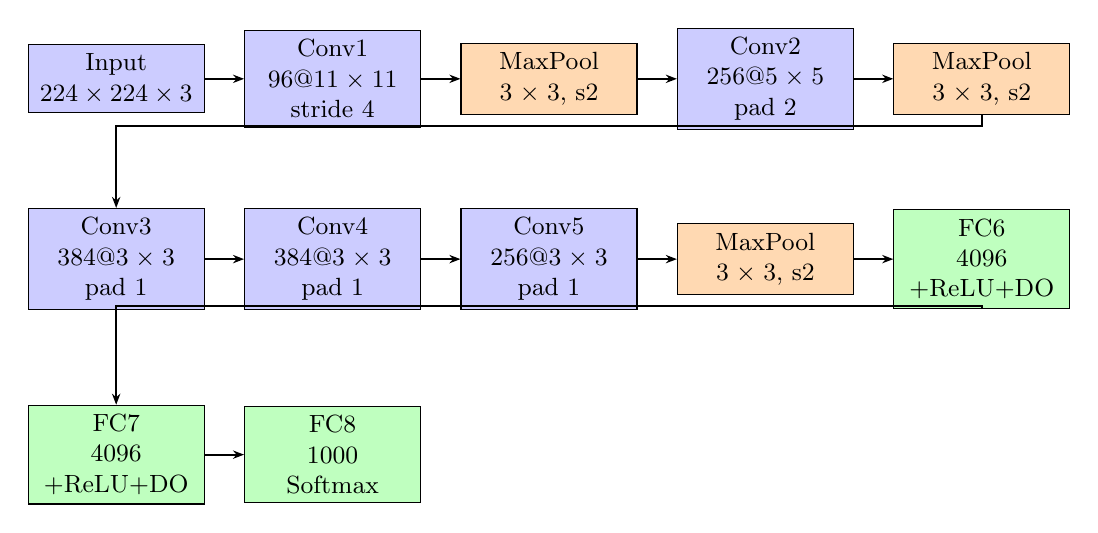
\begin{tikzpicture}[
    node distance=0.6cm and 0.5cm,
    block/.style={rectangle, draw, fill=blue!20, text width=2.0cm, align=center,
                  minimum height=0.7cm, font=\small},
    pool/.style={rectangle, draw, fill=orange!30, text width=2.0cm, align=center,
                 minimum height=0.55cm, font=\small},
    fc/.style={rectangle, draw, fill=green!25, text width=2.0cm, align=center,
               minimum height=0.7cm, font=\small},
    arrow/.style={-{Stealth[length=4pt]}, thick}
  ]
  \node[block] (input) {Input\\$224\times224\times3$};
  \node[block, right=of input] (c1) {Conv1\\96@$11\times11$\\stride 4};
  \node[pool, right=of c1] (p1) {MaxPool\\$3\times3$, s2};
  \node[block, right=of p1] (c2) {Conv2\\256@$5\times5$\\pad 2};
  \node[pool, right=of c2] (p2) {MaxPool\\$3\times3$, s2};
  \node[block, below=1.2cm of input] (c3) {Conv3\\384@$3\times3$\\pad 1};
  \node[block, right=of c3] (c4) {Conv4\\384@$3\times3$\\pad 1};
  \node[block, right=of c4] (c5) {Conv5\\256@$3\times3$\\pad 1};
  \node[pool, right=of c5] (p3) {MaxPool\\$3\times3$, s2};
  \node[fc, right=of p3] (fc6) {FC6\\4096\\+ReLU+DO};
  \node[fc, below=1.2cm of c3] (fc7) {FC7\\4096\\+ReLU+DO};
  \node[fc, right=of fc7] (fc8) {FC8\\1000\\Softmax};

  \draw[arrow] (input) -- (c1);
  \draw[arrow] (c1) -- (p1);
  \draw[arrow] (p1) -- (c2);
  \draw[arrow] (c2) -- (p2);
  \draw[arrow] (p2) -- ++(0,-0.6) -| (c3);
  \draw[arrow] (c3) -- (c4);
  \draw[arrow] (c4) -- (c5);
  \draw[arrow] (c5) -- (p3);
  \draw[arrow] (p3) -- (fc6);
  \draw[arrow] (fc6) -- ++(0,-0.6) -| (fc7);
  \draw[arrow] (fc7) -- (fc8);
\end{tikzpicture}
\caption{AlexNet architecture: five convolutional layers (blue) with max-pooling (orange) followed by three fully-connected layers (green). Dropout is applied at FC6 and FC7.}
\label{fig:alexnet}
\end{figure}

\subsection{Key Innovations}

Four engineering choices enabled AlexNet's success:

\begin{enumerate}[leftmargin=2em]
  \item \textbf{ReLU activation:} $\mathrm{ReLU}(x) = \max(0, x)$ trains several times faster than sigmoid or tanh because it does not saturate in the positive domain and avoids the vanishing gradient problem.
  \begin{equation}
    \mathrm{ReLU}(x) = \max(0,\, x)
    \label{eq:relu}
  \end{equation}
  \item \textbf{Dropout regularization:} With probability $p=0.5$, each neuron in FC6 and FC7 is randomly set to zero during each forward pass of training, preventing co-adaptation of neurons and reducing overfitting.
  \item \textbf{Data augmentation:} Training images are randomly cropped to $224\times224$, horizontally flipped, and perturbed in colour space, artificially increasing the effective dataset size.
  \item \textbf{Multi-GPU training:} The network is split across two NVIDIA GTX 580 GPUs (3 GB memory each), with layers communicating only at selected points. This was essential given the hardware constraints of 2012.
\end{enumerate}

\subsection{ILSVRC Results}

\begin{table}[ht]
\centering
\caption{AlexNet performance on ILSVRC-2010 and ILSVRC-2012 test sets}
\label{tab:alexnet_results}
\begin{tabular}{@{}llcc@{}}
\toprule
Year & Method & Top-1 Error (\%) & Top-5 Error (\%) \\
\midrule
\multirow{3}{*}{2010}
  & Sparse coding (state of the art)   & 47.1 & 28.2 \\
  & SIFT + Fisher vectors (C+FV)        & 45.7 & 25.7 \\
  & AlexNet (1 CNN)                     & 37.5 & 17.0 \\
\midrule
\multirow{2}{*}{2012}
  & Second-best entry (non-DL)          & --   & 26.2 \\
  & AlexNet (ensemble of 7 CNNs)        & --   & 15.3 \\
\bottomrule
\end{tabular}
\end{table}

The gap of $\approx 11$ percentage points in top-5 error at ILSVRC-2012 (from $26.2\%$ to $15.3\%$) was entirely unprecedented in the history of the challenge and immediately attracted worldwide attention to deep learning.

\begin{example}
\textbf{Model ensemble strategy.} The $15.3\%$ top-5 result was achieved by averaging the softmax outputs of seven independently-trained networks: five CNNs with five convolutional layers, one CNN with six convolutional layers, and two CNNs pre-trained on the full ImageNet fall 2011 release. Each network is trained on the same data with slightly different initializations and kernel configurations. Averaging predictions reduces variance and consistently improves accuracy by $1$--$2$ percentage points.
\end{example}

% -------------------------------------------------------
%  4. VGGNET
% -------------------------------------------------------
\section{VGGNet (2014)}
\label{sec:vggnet}

\subsection{Motivation: The Depth Hypothesis}

After the success of AlexNet, researchers asked: \emph{what is the most important architectural dimension -- breadth (number of filters) or depth (number of layers)?} Karen Simonyan and Andrew Zisserman at the Visual Geometry Group (VGG), Oxford, conducted a rigorous investigation: fix all other architectural choices at their simplest values and vary only depth. Their paper, \emph{Very Deep Convolutional Networks for Large-Scale Image Recognition}, appeared at ICLR 2015 \cite{vgg2015}.

\begin{keyinsight}
VGGNet's central contribution is the demonstration that depth using exclusively $3\times3$ convolution filters throughout is the critical factor for achieving strong classification performance. Two stacked $3\times3$ conv layers have the same receptive field as one $5\times5$ layer, but fewer parameters and more non-linearity; three stacked $3\times3$ layers match one $7\times7$ layer, again with fewer parameters.
\end{keyinsight}

\subsection{Receptive Field Analysis}

The effective receptive field equivalence can be verified as follows. Let each $3\times3$ layer apply padding of 1 so that spatial size is preserved. After two such layers, a given output neuron has ``seen'' a $5\times5$ region of the input:
\begin{align}
  r_1 &= 3, \\
  r_2 &= r_1 + (3-1) = 5.
\end{align}
After three layers:
\begin{equation}
  r_3 = 5 + (3-1) = 7.
\end{equation}

Parameter comparison between one $5\times5$ layer and two $3\times3$ layers (both with $C$ channels):
\begin{align}
  \text{Params}(5\times5) &= 5^2 C^2 = 25 C^2, \\
  \text{Params}(2 \times 3\times3) &= 2 \times 3^2 C^2 = 18 C^2.
\end{align}
The two stacked layers use $18/25 = 72\%$ of the parameters and introduce an additional non-linear activation function between them.

\subsection{Architecture Configurations}

VGGNet was evaluated across five depth configurations (A through E). All configurations share:
\begin{itemize}[leftmargin=2em]
  \item Input: $224\times224$ RGB image.
  \item All convolutional filters: $3\times3$, stride 1, padding 1.
  \item Five max-pooling stages: $2\times2$, stride 2.
  \item Three fully-connected layers: FC-4096, FC-4096, FC-1000.
  \item Softmax output for 1000-class classification.
\end{itemize}

The number of convolutional filters doubles with each pooling stage: 64, 128, 256, 512, 512.

\begin{table}[ht]
\centering
\caption{VGGNet configurations A through E with total weight-layer counts and parameter counts}
\label{tab:vgg_configs}
\begin{tabular}{@{}ccccc@{}}
\toprule
Config & Depth (weight layers) & Conv channels & Parameters (M) & Top-5 val.\ error (\%) \\
\midrule
A      & 11 & 64--512 & 133 & 10.4 \\
A-LRN  & 11 & 64--512 & 133 & 10.4 \\
B      & 13 & 64--512 & 133 & 9.9  \\
C      & 16 & 64--512 & 134 & 9.4  \\
D      & 16 & 64--512 & 138 & 8.8  \\
E      & 19 & 64--512 & 144 & 8.7  \\
\bottomrule
\end{tabular}
\end{table}

\noindent Key observation from \cref{tab:vgg_configs}: classification error decreases monotonically as depth increases from 11 to 19 layers, confirming the depth hypothesis. Furthermore, config D (VGG-16) and config E (VGG-19) are the most widely used in practice.

\subsection{Multi-Scale Training}

One important training detail is \emph{multi-scale training}: rather than fixing the training image scale at $S=256$, the scale $S$ is randomly sampled from $[256, 512]$ at each iteration. This acts as a form of scale augmentation, since objects in real images appear at a variety of sizes.

\subsection{ILSVRC Comparison}

\begin{table}[ht]
\centering
\caption{VGGNet vs.\ competing methods on ILSVRC classification (Simonyan \& Zisserman, 2014). Results without external training data only.}
\label{tab:vgg_comparison}
\small
\begin{tabular}{@{}lccc@{}}
\toprule
Method & Top-1 val.\ (\%) & Top-5 val.\ (\%) & Top-5 test (\%) \\
\midrule
VGG (1 net, multi-crop \& dense eval.) -- D  & 24.4 & 7.1  & 7.0 \\
VGG (1 net, multi-crop \& dense eval.) -- E  & 24.7 & 7.5  & 7.3 \\
VGG ILSVRC submission (7 nets, dense)        & 24.7 & 7.5  & 7.1 \\
GoogLeNet (Szegedy et al., 2014) -- 7 nets   & --   & 6.7  & -- \\
MSRA (He et al., 2014) -- 11 nets            & 27.9 & 9.1  & 9.1 \\
Zeiler \& Fergus (2013) -- 6 nets            & 36.0 & 14.7 & 14.8 \\
Zeiler \& Fergus (2013) -- 1 net             & 37.5 & 16.0 & 16.1 \\
OverFeat (Sermanet et al., 2014) -- 1 net    & 34.0 & 13.2 & 13.6 \\
Krizhevsky et al.\ (2012) -- 1 net (AlexNet) & 40.7 & 18.2 & --  \\
\bottomrule
\end{tabular}
\end{table}

\begin{example}
\textbf{Pre-trained model transfer.} A major secondary contribution of VGGNet was demonstrating that features learned on ImageNet transfer well to other visual recognition tasks. Fine-tuning a pre-trained VGG-16 on a target dataset with few samples consistently outperforms training from scratch. This result was instrumental in motivating the large pre-trained model paradigm -- the conceptual precursor to transformer-based foundation models (e.g., BERT, GPT).
\end{example}

\begin{warningbox}
VGGNet's strong performance comes at significant computational cost. VGG-16 has 138 million parameters (compared to AlexNet's 60 million) and requires approximately $15\,\text{GB}$ of memory to train with batch size 256. The three fully-connected layers alone account for the majority of these parameters and most of the inference time. Later architectures (e.g., GoogLeNet, ResNet) achieve better or comparable accuracy with far fewer parameters by eliminating large fully-connected layers.
\end{warningbox}

% -------------------------------------------------------
%  5. RESNET
% -------------------------------------------------------
\section{ResNet (2016)}
\label{sec:resnet}

\subsection{The Degradation Problem}

Following VGGNet's success, the natural question was: \emph{can we keep increasing the depth further?} Experiments with plain networks (no residual connections) revealed a counterintuitive phenomenon: adding more layers beyond a certain threshold actually \emph{increased} both training and test error. This is called the \textbf{degradation problem} and is distinct from overfitting (overfitting would show low training error but high test error).

Kaiming He, Xiangyu Zhang, Shaoqing Ren, and Jian Sun at Microsoft Research addressed this problem in their CVPR 2016 paper \emph{Deep Residual Learning for Image Recognition} \cite{resnet2016}.

\begin{keyinsight}
The degradation problem shows that a 56-layer plain network has \emph{higher training error} than an 18-layer plain network, despite having more capacity. This is not a problem of overfitting -- it is an optimization problem: deep plain networks are simply harder to train. Residual connections solve this by reformulating the learning objective.
\end{keyinsight}

\subsection{Residual Learning Formulation}

In a standard convolutional block, the goal is to learn a mapping $\mathcal{H}(\mathbf{x})$, where $\mathbf{x}$ is the input. ResNet proposes to instead let the stacked non-linear layers fit the \emph{residual function}:
\begin{equation}
  \mathcal{F}(\mathbf{x}) \;=\; \mathcal{H}(\mathbf{x}) - \mathbf{x},
  \label{eq:residual_def}
\end{equation}
so that the desired mapping becomes:
\begin{equation}
  \mathcal{H}(\mathbf{x}) \;=\; \mathcal{F}(\mathbf{x}) + \mathbf{x}.
  \label{eq:residual_mapping}
\end{equation}

This is implemented by a \emph{shortcut connection} (also called a skip connection) that adds the input $\mathbf{x}$ directly to the output of the stacked layers before the final activation:
\begin{equation}
  \mathbf{y} \;=\; \mathcal{F}(\mathbf{x},\, \{W_i\}) + \mathbf{x},
  \label{eq:shortcut}
\end{equation}
where $\{W_i\}$ denotes the weights of the residual branch.

\begin{remark}
If the identity mapping $\mathcal{H}(\mathbf{x}) = \mathbf{x}$ is optimal (i.e., additional layers should not change the representation), it is much easier for the network to push $\mathcal{F}(\mathbf{x}) \to \mathbf{0}$ than to learn the identity function through a stack of non-linear layers. Shortcut connections therefore provide a ``gradient highway'' that allows gradients to flow directly from later layers to earlier layers without passing through non-linearities.
\end{remark}

\subsection{Residual Block Diagram}

\begin{figure}[ht]
\centering
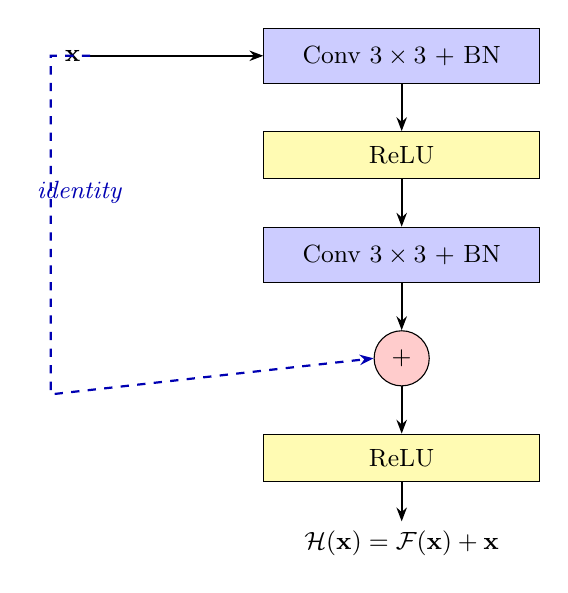
\begin{tikzpicture}[
    node distance=0.8cm,
    conv/.style={rectangle, draw, fill=blue!20, minimum width=3.5cm, minimum height=0.7cm,
                 align=center, font=\small},
    act/.style={rectangle, draw, fill=yellow!30, minimum width=3.5cm, minimum height=0.6cm,
                align=center, font=\small},
    add/.style={circle, draw, fill=red!20, minimum size=0.7cm, font=\small\bfseries},
    arrow/.style={-{Stealth[length=5pt]}, thick}
  ]
  % Main branch
  \node[conv] (conv1) {Conv $3\times3$ + BN};
  \node[act, below=0.6cm of conv1] (relu1) {ReLU};
  \node[conv, below=0.6cm of relu1] (conv2) {Conv $3\times3$ + BN};
  \node[add, below=0.6cm of conv2] (plus) {$+$};
  \node[act, below=0.6cm of plus] (relu2) {ReLU};
  \node[below=0.5cm of relu2, font=\small] (out) {$\mathcal{H}(\mathbf{x}) = \mathcal{F}(\mathbf{x}) + \mathbf{x}$};

  % Skip connection
  \coordinate (skip_start) at ([xshift=-2.5cm]conv1.west);
  \coordinate (skip_end)   at ([xshift=-2.5cm]plus.west);
  \node[left=2.2cm of conv1, font=\small] (x_label) {$\mathbf{x}$};

  \draw[arrow] (x_label) -- (conv1);
  \draw[arrow] (conv1) -- (relu1);
  \draw[arrow] (relu1) -- (conv2);
  \draw[arrow] (conv2) -- (plus);
  \draw[arrow] (plus) -- (relu2);
  \draw[arrow] (relu2) -- (out);

  % Skip path
  \draw[arrow, dashed, blue!70!black, thick]
    (x_label.east) ++(0,0)
    -- ++(-0.5,0)
    -- ++(0,-4.3)
    -- (plus.west);
  \node[above right, font=\small\itshape, blue!70!black] at ([xshift=-3.0cm, yshift=-2.0cm]conv1.west) {identity};
\end{tikzpicture}
\caption{A basic ResNet residual block. The skip connection (dashed blue) adds the input $\mathbf{x}$ directly to the output of the two-layer sub-network, so only the residual $\mathcal{F}(\mathbf{x}) = \mathcal{H}(\mathbf{x}) - \mathbf{x}$ must be learned.}
\label{fig:resblock}
\end{figure}

\subsection{Bottleneck Block}

For deeper variants (ResNet-50/101/152), a \emph{bottleneck} block replaces the basic block to reduce computational cost:
\begin{equation}
  \mathcal{F}(\mathbf{x}) = W_3 \cdot \mathrm{ReLU}(W_2 \cdot \mathrm{ReLU}(W_1 \mathbf{x})),
\end{equation}
where $W_1$ is a $1\times1$ convolution (reducing channels from 256 to 64), $W_2$ is a $3\times3$ convolution, and $W_3$ is a $1\times1$ convolution (expanding back to 256 channels). This $1\times1$--$3\times3$--$1\times1$ pattern processes spatial information at a lower channel dimensionality.

\subsection{Architecture Variants}

\begin{table}[ht]
\centering
\caption{ResNet depth variants: layer composition and top-1 validation error on ILSVRC}
\label{tab:resnet_variants}
\begin{tabular}{@{}lcccc@{}}
\toprule
Variant & Total layers & Block type & Parameters (M) & Top-1 error (\%) \\
\midrule
ResNet-18  & 18  & Basic      & 11.7  & 30.2 \\
ResNet-34  & 34  & Basic      & 21.8  & 26.7 \\
ResNet-50  & 50  & Bottleneck & 25.6  & 24.7 \\
ResNet-101 & 101 & Bottleneck & 44.5  & 23.4 \\
ResNet-152 & 152 & Bottleneck & 60.2  & 23.0 \\
\bottomrule
\end{tabular}
\end{table}

\subsection{Degradation Problem: Quantitative Evidence}

The ResNet paper reported the following comparison on ILSVRC validation:
\begin{itemize}[leftmargin=2em]
  \item Plain-18 top-1 error: $27.94\%$; Plain-34: $28.54\%$ -- \emph{deeper is worse!}
  \item ResNet-18 top-1 error: $27.88\%$; ResNet-34: $25.03\%$ -- \emph{deeper is better.}
\end{itemize}

\subsection{Network Architecture Comparison}

\begin{figure}[ht]
\centering
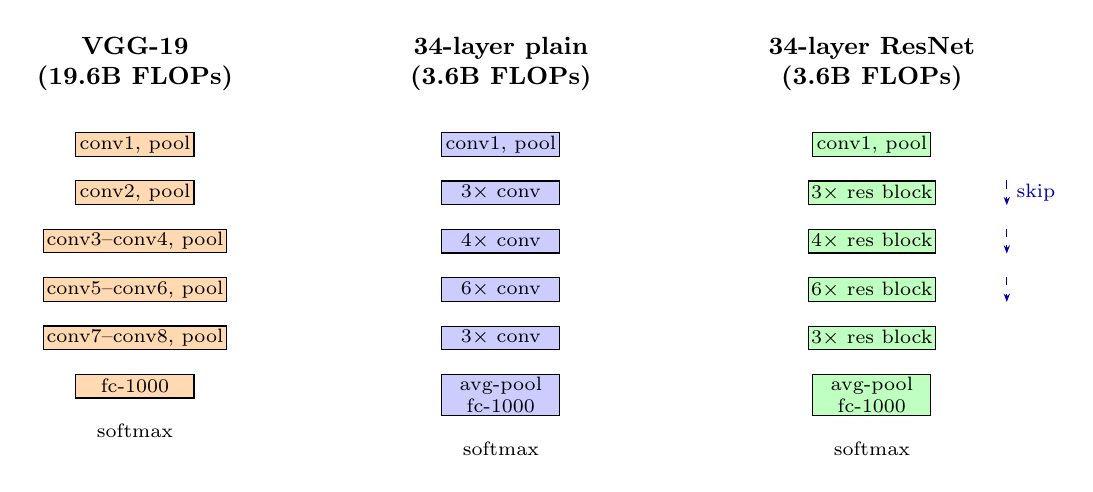
\begin{tikzpicture}[
    node distance=0.3cm and 1.5cm,
    lyr/.style={rectangle, draw, minimum width=1.5cm, minimum height=0.3cm, align=center,
                font=\scriptsize, inner sep=1pt},
    vgg/.style={lyr, fill=orange!30},
    plain/.style={lyr, fill=blue!20},
    res/.style={lyr, fill=green!25},
    title/.style={font=\small\bfseries, align=center},
    arrow/.style={-{Stealth[length=4pt]}, thick}
  ]

  % --- VGG-19 column ---
  \node[title] (vtitle) {VGG-19\\(19.6B FLOPs)};
  \node[vgg, below=0.4cm of vtitle] (v1) {conv1, pool};
  \node[vgg, below=of v1] (v2) {conv2, pool};
  \node[vgg, below=of v2] (v3) {conv3--conv4, pool};
  \node[vgg, below=of v3] (v4) {conv5--conv6, pool};
  \node[vgg, below=of v4] (v5) {conv7--conv8, pool};
  \node[vgg, below=of v5] (v6) {fc-1000};
  \node[below=0.2cm of v6, font=\scriptsize] {softmax};

  % --- 34-layer plain ---
  \node[title, right=2.0cm of vtitle] (ptitle) {34-layer plain\\(3.6B FLOPs)};
  \node[plain, below=0.4cm of ptitle] (p1) {conv1, pool};
  \node[plain, below=of p1] (p2) {$3\times$ conv};
  \node[plain, below=of p2] (p3) {$4\times$ conv};
  \node[plain, below=of p3] (p4) {$6\times$ conv};
  \node[plain, below=of p4] (p5) {$3\times$ conv};
  \node[plain, below=of p5] (p6) {avg-pool\\fc-1000};
  \node[below=0.2cm of p6, font=\scriptsize] {softmax};

  % --- 34-layer residual ---
  \node[title, right=2.0cm of ptitle] (rtitle) {34-layer ResNet\\(3.6B FLOPs)};
  \node[res, below=0.4cm of rtitle] (r1) {conv1, pool};
  \node[res, below=of r1] (r2) {$3\times$ res block};
  \node[res, below=of r2] (r3) {$4\times$ res block};
  \node[res, below=of r3] (r4) {$6\times$ res block};
  \node[res, below=of r4] (r5) {$3\times$ res block};
  \node[res, below=of r5] (r6) {avg-pool\\fc-1000};
  \node[below=0.2cm of r6, font=\scriptsize] {softmax};

  % Skip connection arrows on residual column
  \draw[-{Stealth[length=3pt]}, dashed, blue!70!black]
    ([xshift=0.9cm]r2.north east) -- ([xshift=0.9cm]r2.south east)
    node[midway, right, font=\scriptsize, blue!70!black] {skip};
  \draw[-{Stealth[length=3pt]}, dashed, blue!70!black]
    ([xshift=0.9cm]r3.north east) -- ([xshift=0.9cm]r3.south east);
  \draw[-{Stealth[length=3pt]}, dashed, blue!70!black]
    ([xshift=0.9cm]r4.north east) -- ([xshift=0.9cm]r4.south east);
\end{tikzpicture}
\caption{Side-by-side comparison of VGG-19, 34-layer plain network, and 34-layer ResNet. The residual network uses significantly fewer FLOPs than VGG-19 while achieving better accuracy. Skip connections (dashed blue) bypass pairs of layers in the residual network.}
\label{fig:arch_comparison}
\end{figure}

% -------------------------------------------------------
%  6. ALGORITHMS
% -------------------------------------------------------
\section{Training Algorithms}
\label{sec:algorithms}

\subsection{Standard CNN Training with SGD}

\begin{algorithm}[H]
\caption{Stochastic Gradient Descent Training for CNN Classification}
\label{alg:sgd_cnn}
\SetAlgoLined
\DontPrintSemicolon
\KwIn{Training set $\mathcal{D} = \{(\mathbf{x}_i, y_i)\}_{i=1}^N$, CNN $f_\theta$, learning rate $\eta$, momentum $\mu$, weight decay $\lambda$, epochs $T$}
\KwOut{Optimized parameters $\theta^*$}
Initialize $\theta$ (e.g., He initialization for ReLU networks)\;
$\mathbf{v} \leftarrow \mathbf{0}$ \tcp*{momentum buffer}
\For{$t = 1, 2, \ldots, T$}{
  Shuffle $\mathcal{D}$ into mini-batches $\mathcal{B}_1, \mathcal{B}_2, \ldots$\;
  \For{each mini-batch $\mathcal{B}$}{
    Forward pass: compute logits $\hat{\mathbf{y}} = f_\theta(\mathbf{x})$ for $\mathbf{x} \in \mathcal{B}$\;
    Compute cross-entropy loss:
    $\mathcal{L} = -\dfrac{1}{|\mathcal{B}|}\sum_{(\mathbf{x},y) \in \mathcal{B}} \log \hat{p}_y + \lambda \|\theta\|^2_2$\;
    Backward pass: compute $\mathbf{g} = \nabla_\theta \mathcal{L}$\;
    Update momentum: $\mathbf{v} \leftarrow \mu\,\mathbf{v} + \mathbf{g}$\;
    Update parameters: $\theta \leftarrow \theta - \eta\,\mathbf{v}$\;
  }
  Decay $\eta$ if validation loss plateaus\;
}
\Return $\theta$\;
\end{algorithm}

\subsection{Data Augmentation Strategy}

Both AlexNet and VGGNet use the following data augmentation during training:
\begin{enumerate}[leftmargin=2em]
  \item \textbf{Random crop:} From a rescaled image, randomly extract a $224\times224$ patch.
  \item \textbf{Horizontal flip:} With probability 0.5, flip the patch left-right.
  \item \textbf{Colour jitter (AlexNet only):} Add multiples of the principal components of the RGB pixel values across the training set, sampled from $\mathcal{N}(0, 0.1)$.
  \item \textbf{Multi-scale jitter (VGGNet only):} Randomly sample the rescaling factor $S \in [256, 512]$ before cropping.
\end{enumerate}

During test time, standard practice is to evaluate on 10 crops (4 corners + centre, $\times$ 2 for horizontal flip) and average the softmax outputs.

% -------------------------------------------------------
%  7. COMPARATIVE ANALYSIS
% -------------------------------------------------------
\section{Comparative Analysis and Historical Progression}
\label{sec:comparison}

\subsection{Error Rate Progression on ILSVRC}

The following diagram summarizes the historical progression:

\begin{figure}[ht]
\centering
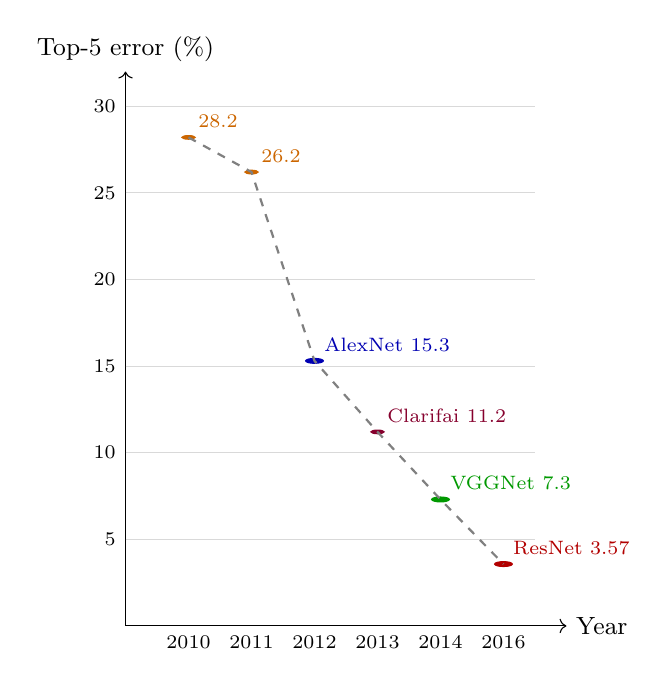
\begin{tikzpicture}
  \begin{scope}[xscale=0.8, yscale=0.22]
    % Axes
    \draw[->] (0,0) -- (7,0) node[right, font=\small] {Year};
    \draw[->] (0,0) -- (0,32) node[above, font=\small] {Top-5 error (\%)};

    % Grid lines
    \foreach \y in {5,10,15,20,25,30} {
      \draw[gray!30] (0,\y) -- (6.5,\y);
      \node[left, font=\scriptsize] at (0,\y) {\y};
    }

    % Year labels
    \foreach \x/\lbl in {1/2010, 2/2011, 3/2012, 4/2013, 5/2014, 6/2016} {
      \node[below, font=\scriptsize] at (\x,0) {\lbl};
    }

    % Prior methods (pre-2012)
    \filldraw[orange!80!black] (1,28.2) circle (3pt) node[above right, font=\scriptsize]{28.2};
    \filldraw[orange!80!black] (2,26.2) circle (3pt) node[above right, font=\scriptsize]{26.2};

    % AlexNet 2012
    \filldraw[blue!70!black] (3,15.3) circle (4pt) node[above right, font=\scriptsize]{AlexNet 15.3};

    % 2013 improvements
    \filldraw[purple!70!black] (4,11.2) circle (3pt) node[above right, font=\scriptsize]{Clarifai 11.2};

    % VGGNet 2014
    \filldraw[green!60!black] (5,7.3) circle (4pt) node[above right, font=\scriptsize]{VGGNet 7.3};

    % ResNet 2016
    \filldraw[red!70!black] (6,3.57) circle (4pt) node[above right, font=\scriptsize]{ResNet 3.57};

    % Connect the dots
    \draw[thick, dashed, gray]
      (1,28.2) -- (2,26.2) -- (3,15.3) -- (4,11.2) -- (5,7.3) -- (6,3.57);
  \end{scope}
\end{tikzpicture}
\caption{Top-5 error rate on ILSVRC from 2010 to 2016. The steep drop from 2011 to 2012 marks the arrival of AlexNet. VGGNet and ResNet continued the trajectory, with ResNet (ensemble) reaching $3.57\%$ -- surpassing estimated human-level performance of approximately $5\%$.}
\label{fig:error_progression}
\end{figure}

\subsection{Architecture Comparison Table}

\begin{table}[ht]
\centering
\caption{Summary comparison of AlexNet, VGGNet, and ResNet architectures}
\label{tab:arch_summary}
\begin{tabular}{@{}lccccc@{}}
\toprule
Architecture & Year & Depth & Params (M) & ILSVRC Top-5 (\%) & Key Innovation \\
\midrule
AlexNet  & 2012 & 8   & 60  & 15.3 & ReLU, Dropout, GPU \\
VGGNet-16 & 2014 & 16  & 138 & 7.3  & Depth with $3\times3$ \\
VGGNet-19 & 2014 & 19  & 144 & 7.0  & Depth with $3\times3$ \\
ResNet-34  & 2016 & 34  & 22  & 7.4  & Residual connections \\
ResNet-50  & 2016 & 50  & 26  & 6.7  & Bottleneck blocks \\
ResNet-152 & 2016 & 152 & 60  & 5.7  & Extreme depth \\
ResNet ens. & 2016 & --  & --  & 3.57 & Ensemble of ResNets \\
\bottomrule
\end{tabular}
\end{table}

\subsection{Design Philosophy Comparison}

Each architecture embodies a distinct design philosophy:

\begin{itemize}[leftmargin=2em]
  \item \textbf{AlexNet:} ``More capacity via moderate depth + many filters + powerful hardware.'' Introduced the toolkit (ReLU, Dropout, data augmentation, GPU) that all subsequent architectures rely on.
  \item \textbf{VGGNet:} ``Depth with small filters is the key factor.'' Showed that a uniform $3\times3$ filter strategy, pushed to 16--19 layers, outperforms shallower architectures with larger filters and more parameters.
  \item \textbf{ResNet:} ``Residual learning solves the optimization problem of very deep networks.'' The key insight is not just depth but \emph{trainable depth}: skip connections make it possible to reliably optimize networks with hundreds of layers.
\end{itemize}

\begin{keyinsight}
The transition from AlexNet to VGGNet to ResNet reflects a general principle in deep learning: \emph{depth is more important than breadth for representational power}, but only when the optimization problem associated with deep networks is properly addressed. ResNet's residual formulation is the solution to that optimization problem.
\end{keyinsight}

% -------------------------------------------------------
%  8. MATHEMATICAL DETAILS
% -------------------------------------------------------
\section{Mathematical Details}
\label{sec:math}

\subsection{Convolutional Layer Forward Pass}

Given an input feature map $\mathbf{X} \in \mathbb{R}^{H \times W \times C_{\text{in}}}$ and a filter bank $\mathbf{W} \in \mathbb{R}^{K \times K \times C_{\text{in}} \times C_{\text{out}}}$ with bias $\mathbf{b} \in \mathbb{R}^{C_{\text{out}}}$, the output at spatial location $(i,j)$ for output channel $k$ is:
\begin{equation}
  \mathbf{Y}_{i,j,k} = b_k + \sum_{c=1}^{C_{\text{in}}} \sum_{p=0}^{K-1} \sum_{q=0}^{K-1}
    \mathbf{W}_{p,q,c,k} \cdot \mathbf{X}_{i\cdot s + p,\, j\cdot s + q,\, c},
  \label{eq:conv}
\end{equation}
where $s$ is the stride.

\subsection{Batch Normalization}

ResNet layers include Batch Normalization (BN) after each convolution and before each activation:
\begin{align}
  \hat{x}_i &= \frac{x_i - \mu_\mathcal{B}}{\sqrt{\sigma^2_\mathcal{B} + \epsilon}},
  \label{eq:bn_norm}\\
  y_i &= \gamma \hat{x}_i + \beta,
  \label{eq:bn_scale}
\end{align}
where $\mu_\mathcal{B}$ and $\sigma^2_\mathcal{B}$ are the mini-batch mean and variance, and $\gamma$, $\beta$ are learned scale and shift parameters. BN accelerates training by reducing internal covariate shift and allows higher learning rates.

\subsection{Cross-Entropy Loss with Softmax}

For a $C$-class classification problem, the model outputs a logit vector $\mathbf{z} \in \mathbb{R}^C$. The softmax function converts logits to probabilities:
\begin{equation}
  \hat{p}_c = \frac{e^{z_c}}{\sum_{j=1}^{C} e^{z_j}},
  \qquad c = 1, \ldots, C.
  \label{eq:softmax}
\end{equation}
The cross-entropy loss for a batch of $N$ samples is:
\begin{equation}
  \mathcal{L} = -\frac{1}{N} \sum_{i=1}^{N} \log \hat{p}_{y_i},
  \label{eq:ce_loss}
\end{equation}
where $y_i$ is the ground-truth class label for sample $i$.

\subsection{L2 Regularization and Effective Learning}

All three architectures use L2 weight decay (equivalent to a Gaussian prior on weights):
\begin{equation}
  \mathcal{L}_{\text{reg}} = \mathcal{L}_{\text{CE}} + \frac{\lambda}{2} \|\theta\|^2_2,
  \label{eq:l2_reg}
\end{equation}
where $\lambda$ is the weight decay coefficient (typically $5\times10^{-4}$ for AlexNet and VGGNet, $10^{-4}$ for ResNet).

% -------------------------------------------------------
%  9. SUMMARY
% -------------------------------------------------------
\section{Summary}
\label{sec:summary}

Session 14 traced the arc of CNN architecture development from the AlexNet breakthrough of 2012 to the ResNet ensemble result of 2016 -- a trajectory that reduced ILSVRC top-5 error from $26.2\%$ to $3.57\%$ in four years.

\paragraph{AlexNet (NIPS 2012).}
Five convolutional layers and three fully-connected layers; 60 million parameters; trained on two GPUs. Key innovations: ReLU activations for faster training, Dropout for regularization, and data augmentation. Achieved $15.3\%$ top-5 error at ILSVRC-2012, an $11$ percentage point improvement over the non-deep-learning runner-up.

\paragraph{VGGNet (ICLR 2015).}
Depth-first exploration using exclusively $3\times3$ filters. Configurations from 11 to 19 weight layers, all with 64--512 filters doubling after each pooling. Achieved $7.3\%$ top-5 test error (VGG-16) and $7.0\%$ (VGG-19) at ILSVRC-2014. Introduced the concept of deep, pre-trained CNN features that generalize to other tasks -- a precursor to transfer learning.

\paragraph{ResNet (CVPR 2016).}
Introduced residual (skip) connections to address the \emph{degradation problem}: plain networks with more than $\sim$20 layers exhibited \emph{higher} training error than shallower networks. The residual formulation $\mathcal{H}(\mathbf{x}) = \mathcal{F}(\mathbf{x}) + \mathbf{x}$ made it possible to train networks with 34, 50, 101, and 152 layers, achieving $5.7\%$ top-5 error with ResNet-152 and $3.57\%$ with an ensemble -- surpassing human-level performance on ILSVRC for the first time.

\medskip

These three architectures established the foundational design patterns of modern deep learning: ReLU activations, batch normalization, residual connections, and depth-first design. They remain the backbone of countless production systems and the starting point for new research across vision, speech, and beyond.

\begin{keyinsight}
The Instructor's recommendation: read all three original papers -- Krizhevsky et al.\ (2012), Simonyan \& Zisserman (2014), and He et al.\ (2016) -- not only for their technical content but for the clarity of their experimental methodology and the impact of their results on the trajectory of the entire field.
\end{keyinsight}

% -------------------------------------------------------
%  APPENDIX A: PRACTICAL NOTES AND TRANSFER LEARNING
% -------------------------------------------------------
\section{Practical Notes: Transfer Learning and Pre-trained Models}
\label{sec:transfer}

\subsection{The Pre-trained Model Paradigm}

One of the most practically significant outcomes of the VGGNet and ResNet era was the establishment of the \emph{pre-trained model} paradigm. The core idea is:

\begin{enumerate}[leftmargin=2em]
  \item Train a deep CNN on a very large labelled dataset (e.g., ImageNet with 1.2 million images).
  \item Use the learned weights as a starting point (``initialization'') for a related task where labelled data is scarce.
  \item \emph{Fine-tune} some or all of the network's weights on the target task.
\end{enumerate}

This approach is justified by the observation that the lower layers of a deep CNN learn general-purpose visual features (edges, textures, colour blobs) that are broadly useful across many visual tasks, while only the upper layers specialize to the specific classes in the training dataset.

\begin{example}
\textbf{Medical image analysis using VGG-16 transfer learning.} Suppose a hospital has 5000 labelled chest X-rays (``normal'' vs.\ ``pneumonia''). Training a deep CNN from scratch on 5000 images is likely to overfit. Instead:
\begin{enumerate}[leftmargin=2em]
  \item Download VGG-16 pre-trained on ImageNet.
  \item Replace the final FC-1000 layer with FC-2 (two output classes).
  \item Freeze weights in Conv1--Conv3 (general low-level features).
  \item Fine-tune Conv4, Conv5, and the new FC layers at a low learning rate ($10^{-5}$).
\end{enumerate}
This typically achieves accuracy 10--15\% higher than training from scratch, despite the ImageNet pre-training data containing no medical images.
\end{example}

\subsection{Feature Extraction vs.\ Fine-Tuning}

Two standard strategies exist for applying pre-trained models:

\begin{table}[ht]
\centering
\caption{Comparison of feature extraction and fine-tuning strategies for transfer learning}
\label{tab:transfer_strategies}
\begin{tabular}{@{}lcccc@{}}
\toprule
Strategy & Frozen layers & Trainable layers & Data required & Computation \\
\midrule
Feature extraction & All conv layers & FC layers only & Very small & Low \\
Partial fine-tuning & Conv1--Conv3 & Conv4+, FC & Small--medium & Medium \\
Full fine-tuning & None & All layers & Large & High \\
\bottomrule
\end{tabular}
\end{table}

\subsection{Why Residual Networks Changed Everything}

The success of ResNet had a broader impact beyond ILSVRC. The residual connection principle was quickly adopted in:

\begin{itemize}[leftmargin=2em]
  \item \textbf{Object detection:} Faster R-CNN with ResNet backbone replaced VGG.
  \item \textbf{Semantic segmentation:} DeepLab and FCN architectures adopted residual backbones.
  \item \textbf{Natural language processing:} The Transformer architecture (2017) uses residual connections in both the encoder and decoder, explicitly crediting the ResNet design.
  \item \textbf{Speech processing:} Deep residual networks for acoustic modeling followed the ResNet paper.
\end{itemize}

\begin{remark}
The instructor noted that VGGNet's demonstration of powerful pre-trained features directly motivated the development of transformer-based large pre-trained models (BERT, GPT, etc.\ for NLP). The question ``can we have an equivalent of VGGNet/ResNet for sequence data?'' led to the proposal and rapid adoption of the Transformer architecture.
\end{remark}

% -------------------------------------------------------
%  APPENDIX B: GRADIENT FLOW IN DEEP NETWORKS
% -------------------------------------------------------
\section{Gradient Flow Analysis}
\label{sec:gradient_flow}

\subsection{Vanishing Gradients in Plain Networks}

For a plain $L$-layer network without skip connections, the gradient of the loss $\mathcal{L}$ with respect to weights at layer $\ell$ is:
\begin{equation}
  \frac{\partial \mathcal{L}}{\partial W_\ell}
  = \frac{\partial \mathcal{L}}{\partial \mathbf{z}_L}
    \cdot \prod_{k=\ell+1}^{L} \frac{\partial \mathbf{z}_k}{\partial \mathbf{z}_{k-1}}
    \cdot \frac{\partial \mathbf{z}_\ell}{\partial W_\ell},
  \label{eq:chain_rule}
\end{equation}
where $\mathbf{z}_k$ is the pre-activation at layer $k$. Each Jacobian $\frac{\partial \mathbf{z}_k}{\partial \mathbf{z}_{k-1}}$ depends on the weight matrix and the activation derivative. For ReLU activations and poorly conditioned weight matrices, these Jacobians have singular values that are typically $< 1$, so the product in \cref{eq:chain_rule} decays exponentially with depth, causing \emph{vanishing gradients}.

\subsection{Gradient Flow Through Skip Connections}

For a residual block $\mathbf{y} = \mathcal{F}(\mathbf{x}) + \mathbf{x}$, the gradient with respect to the input $\mathbf{x}$ is:
\begin{equation}
  \frac{\partial \mathcal{L}}{\partial \mathbf{x}}
  = \frac{\partial \mathcal{L}}{\partial \mathbf{y}}
    \cdot \left(\frac{\partial \mathcal{F}(\mathbf{x})}{\partial \mathbf{x}} + \mathbf{I}\right),
  \label{eq:resgrad}
\end{equation}
where $\mathbf{I}$ is the identity matrix. The identity term guarantees that even if $\frac{\partial \mathcal{F}}{\partial \mathbf{x}} \approx \mathbf{0}$ (the residual branch contributes little to learning), the gradient $\frac{\partial \mathcal{L}}{\partial \mathbf{x}}$ is still approximately $\frac{\partial \mathcal{L}}{\partial \mathbf{y}}$ -- not attenuated. This is the mathematical reason that residual networks can be trained successfully to arbitrary depth.

\begin{theorem}[Gradient Propagation Bound for ResNets]
\label{thm:resnet_grad}
Consider a residual network with $L$ blocks, each satisfying $\mathbf{y}_\ell = \mathcal{F}_\ell(\mathbf{x}_\ell) + \mathbf{x}_\ell$. Expanding the chain rule recursively, the gradient at any intermediate layer $\ell$ contains a direct sum-path from the output:
\begin{equation}
  \frac{\partial \mathcal{L}}{\partial \mathbf{x}_\ell}
  = \frac{\partial \mathcal{L}}{\partial \mathbf{x}_L}
    \cdot \left(\mathbf{I} + \sum_{k=\ell}^{L-1} \prod_{j=k}^{L-1}
      \frac{\partial \mathcal{F}_j}{\partial \mathbf{x}_j}\right).
  \label{eq:resnet_grad_bound}
\end{equation}
The identity term $\mathbf{I}$ ensures that the gradient never vanishes to zero, regardless of the depth $L$ or the magnitudes of the residual Jacobians.
\end{theorem}

\subsection{He Initialization}

To complement residual learning, He et al.\ proposed a weight initialization scheme designed for ReLU networks:
\begin{equation}
  W \sim \mathcal{N}\!\left(0,\, \frac{2}{n_{\text{in}}}\right),
  \label{eq:he_init}
\end{equation}
where $n_{\text{in}}$ is the fan-in (number of input units to the layer). This initialization preserves the variance of activations through the forward pass and of gradients through the backward pass for ReLU networks, enabling stable training from the very start.

\begin{warningbox}
Using the Glorot/Xavier initialization (designed for tanh/sigmoid) with ReLU networks causes activations to diminish in deep networks because it does not account for the factor of $1/2$ introduced by the ReLU non-linearity (which zeros out half of all activations on average). He initialization corrects for this by doubling the variance.
\end{warningbox}

% -------------------------------------------------------
%  APPENDIX C: REVIEW QUESTIONS
% -------------------------------------------------------
\section{Review Questions}
\label{sec:review}

The following questions test understanding of the key concepts from Session 14.

\begin{enumerate}[leftmargin=2em, label=\textbf{Q\arabic*.}]

  \item \textbf{Top-$k$ error.}
  A model outputs the following class probabilities for a test image with true label ``cat'' (class 3):
  \[
    [\underbrace{0.4}_{\text{class 1}},\; \underbrace{0.3}_{\text{class 2}},\;
     \underbrace{0.15}_{\text{class 3}},\; \underbrace{0.1}_{\text{class 4}},\;
     \underbrace{0.05}_{\text{class 5}}]
  \]
  Compute the top-1 error and top-5 error for this prediction.

  \item \textbf{Receptive field.}
  Show that three stacked $3\times3$ convolutional layers (stride 1, padding 1) have the same receptive field as one $7\times7$ layer. How many parameters does each require for $C=128$ input and output channels?

  \item \textbf{Degradation problem.}
  A plain 56-layer network has higher training error than an 18-layer network on the same dataset. Is this evidence of: (a) overfitting, (b) underfitting, or (c) an optimization problem? Justify your answer.

  \item \textbf{Residual learning.}
  Suppose a residual block learns $\mathcal{F}(\mathbf{x}) = \mathbf{0}$. What does the block output? What does this imply about the ability of residual networks to represent shallower functions?

  \item \textbf{Transfer learning.}
  You have a dataset of 10,000 satellite images labelled as ``urban'' or ``non-urban''. Would you prefer to: (a) train a ResNet-50 from scratch, (b) use ResNet-50 features with a linear classifier, or (c) fine-tune the top half of a pre-trained ResNet-50? Justify your choice.

  \item \textbf{Parameter count.}
  AlexNet's fully-connected layers (FC6, FC7, FC8) contain approximately how many of the 60 million total parameters? (Hint: FC6 input is $6\times6\times256=9216$ units; FC6 has 4096 neurons; FC7 has 4096 neurons; FC8 has 1000 neurons.)

\end{enumerate}

% -------------------------------------------------------
%  APPENDIX D: VGGNET DEPTH CONFIGURATIONS -- DETAILED
% -------------------------------------------------------
\section{VGGNet Depth Configurations in Detail}
\label{sec:vgg_detail}

\subsection{Filter Progression and Spatial Dimensions}

The following traces the spatial dimensions and filter counts for VGG-16 (configuration D):

\begin{table}[ht]
\centering
\caption{VGG-16 (configuration D) layer-by-layer spatial and channel dimensions}
\label{tab:vgg16_detail}
\small
\begin{tabular}{@{}clccc@{}}
\toprule
Stage & Layers & Input size & Filters & Output size \\
\midrule
1 & Conv3-64, Conv3-64, MaxPool & $224\times224\times3$   & 64  & $112\times112\times64$ \\
2 & Conv3-128, Conv3-128, MaxPool & $112\times112\times64$  & 128 & $56\times56\times128$ \\
3 & Conv3-256 $\times3$, MaxPool & $56\times56\times128$   & 256 & $28\times28\times256$ \\
4 & Conv3-512 $\times3$, MaxPool & $28\times28\times256$   & 512 & $14\times14\times512$ \\
5 & Conv3-512 $\times3$, MaxPool & $14\times14\times512$   & 512 & $7\times7\times512$ \\
6 & FC-4096, FC-4096, FC-1000    & $7\times7\times512=25088$ & -- & 1000 \\
\bottomrule
\end{tabular}
\end{table}

\subsection{Why 1$\times$1 Convolutions Appear in Config C}

Configuration C introduces $1\times1$ convolution layers in addition to $3\times3$ layers. A $1\times1$ convolution applies a linear transformation to the channel dimension at each spatial location independently:
\begin{equation}
  \mathbf{Y}_{i,j,k} = \sum_{c=1}^{C_{\text{in}}} W_{c,k} \cdot \mathbf{X}_{i,j,c}.
  \label{eq:1x1conv}
\end{equation}
This is equivalent to a fully-connected layer applied channel-wise, allowing the network to increase non-linearity (by adding an extra ReLU) without increasing the spatial receptive field. The VGGNet paper found that config D (no $1\times1$ convolutions) outperformed config C (with $1\times1$ convolutions) at the same depth, confirming that spatial context captured by $3\times3$ filters is more important than additional non-linearity from $1\times1$ filters.

\subsection{Multi-Scale Testing}

At test time, VGGNet applies the network at multiple scales $Q \in \{S-32, S, S+32\}$ (where $S$ is the training scale) and averages the resulting class score maps. This is called \emph{dense evaluation} and differs from the simpler multi-crop evaluation used by AlexNet. Dense evaluation converts FC layers to $1\times1$ convolutional layers, allowing the network to process images of arbitrary size and produce a spatial score map rather than a single vector.

\begin{example}
\textbf{Dense vs.\ multi-crop evaluation.}
For a test image of size $384\times384$ (with $S=256$ training scale):
\begin{itemize}[leftmargin=2em]
  \item \emph{Multi-crop:} Extract 10 crops of size $224\times224$, classify each, average.
  \item \emph{Dense:} Convert FC to $1\times1$ conv, apply to full $384\times384$ image. The network outputs a $6\times6\times1000$ score map. Average over the $36$ spatial positions.
\end{itemize}
Dense evaluation is more computationally efficient than multi-crop because computations are shared between overlapping receptive fields.
\end{example}

% -------------------------------------------------------
%  APPENDIX E: RESNET BOTTLENECK AND IDENTITY SHORTCUTS
% -------------------------------------------------------
\section{ResNet Bottleneck Blocks and Projection Shortcuts}
\label{sec:resnet_bottleneck}

\subsection{When Skip Connections Need Projection}

In the basic ResNet formulation, the skip connection performs an identity mapping: $\mathbf{y} = \mathcal{F}(\mathbf{x}) + \mathbf{x}$. This requires $\mathbf{x}$ and $\mathcal{F}(\mathbf{x})$ to have the same dimensions. When the number of channels or spatial dimensions change (e.g., when transitioning between stages), a \emph{projection shortcut} is used:
\begin{equation}
  \mathbf{y} = \mathcal{F}(\mathbf{x},\, \{W_i\}) + W_s \mathbf{x},
  \label{eq:projection_shortcut}
\end{equation}
where $W_s$ is a $1\times1$ convolutional projection that matches dimensions. In ResNet-50/101/152, projection shortcuts are used only when dimensions change; all other skip connections remain identity mappings.

\subsection{Bottleneck Parameter Count}

For a bottleneck block with $d=256$ input/output channels and $d'=64$ bottleneck channels:
\begin{align}
  \text{Params}(\text{bottleneck}) &= d \cdot d' \cdot 1^2 + d' \cdot d' \cdot 3^2 + d' \cdot d \cdot 1^2 \notag \\
  &= 256 \cdot 64 + 64 \cdot 64 \cdot 9 + 64 \cdot 256 \notag \\
  &= 16384 + 36864 + 16384 = 69632.
  \label{eq:bottleneck_params}
\end{align}
For comparison, a basic block with two $3\times3$ convolutions at $d=256$ channels requires:
\begin{equation}
  \text{Params}(\text{basic}) = 2 \times 256 \times 256 \times 9 = 1{,}179{,}648.
  \label{eq:basic_params}
\end{equation}
The bottleneck reduces parameter count by a factor of approximately 17, enabling much greater depth at the same computational budget.

\begin{keyinsight}
The bottleneck design principle -- compress to a lower-dimensional representation, process spatially, then expand -- recurs throughout modern deep learning: it appears in MobileNet's depthwise separable convolutions, in the Transformer's feed-forward sublayer ($d_{\text{model}} \to 4 d_{\text{model}} \to d_{\text{model}}$), and in the inverted residual blocks of MobileNetV2.
\end{keyinsight}

% -------------------------------------------------------
%  REFERENCES
% -------------------------------------------------------
\begin{thebibliography}{9}

\bibitem{alexnet2012}
Alex Krizhevsky, Ilya Sutskever, and Geoffrey E.\ Hinton.
\newblock ImageNet Classification with Deep Convolutional Neural Networks.
\newblock In \emph{Advances in Neural Information Processing Systems (NIPS)}, 2012.

\bibitem{vgg2015}
Karen Simonyan and Andrew Zisserman.
\newblock Very Deep Convolutional Networks for Large-Scale Image Recognition.
\newblock In \emph{International Conference on Learning Representations (ICLR)}, 2015.

\bibitem{resnet2016}
Kaiming He, Xiangyu Zhang, Shaoqing Ren, and Jian Sun.
\newblock Deep Residual Learning for Image Recognition.
\newblock In \emph{Proceedings of the IEEE Conference on Computer Vision and Pattern Recognition (CVPR)}, 2016.

\bibitem{zeiler2013}
Matthew D.\ Zeiler and Rob Fergus.
\newblock Visualizing and Understanding Convolutional Networks.
\newblock In \emph{European Conference on Computer Vision (ECCV)}, 2014.

\bibitem{overfeat2014}
Pierre Sermanet, David Eigen, Xiang Zhang, Michael Mathieu, Rob Fergus, and Yann LeCun.
\newblock OverFeat: Integrated Recognition, Localization and Detection using Convolutional Networks.
\newblock In \emph{ICLR}, 2014.

\end{thebibliography}

\end{document}
